\documentclass[a4paper]{article}

\usepackage[utf8]{inputenc}
\usepackage[T1]{fontenc}
\usepackage{lipsum}
\usepackage{enumitem,kantlipsum}
\usepackage{verbatim}
\usepackage{graphicx}

\graphicspath{ {images/} }

\title{Pollution Detection System\\User Manual}
\author{PLA25}

\begin{document}

\maketitle
\vspace*{\fill}

\paragraph{Group members}
\begin{tabbing}
	Joey Blankendaal 	\` 	500778751 	\\
	Thom de Jong 		\` 	500778147 	\\
	Brian Karmelk 		\` 	500768939 	\\
	Matthijs Snijders 	\` 	500780453 	\\
	Rico Snoek 			\` 	500778357 	\\
	Martijn Vegter 		\` 	500775388
\end{tabbing}

\thispagestyle{empty}
\pagebreak

\tableofcontents
\pagebreak

\section{Introduction}

\subsection{Who are we?}
We are a group of students who go by the name of PLA25. We visit the HvA, in Amsterdam.

\subsection{Our product}
The Pollution Detection System is a web-based application that provides information about the pollution on earth. Both light pollution and air pollution are being monitored using this system.
\newline
The system uses so called "sensorhubs". Sensorhubs are a combination of multiple sensors inside of a box. These sensorhubs can be placed in a specific area to measure the pollution. These measurements can be monitored using the PDS website. This can be done by using the website's main feature, the map.
The system uses sensors that can be placed in a specific area to measure the pollution. These measurements can be monitored using the PDS website. This can be done by using the website's main feature, the map.

\pagebreak

\section{The website}
\subsection{Login and Logout}
The login page is simple, use your username and password to login to the website.

\begin{enumerate}[wide, labelwidth=!, labelindent=0pt]
	\item Use the upper input field for your username.
	\item Use the lower one for your password.
	\item Finally, click the "login" button.
\end{enumerate}

\noindent
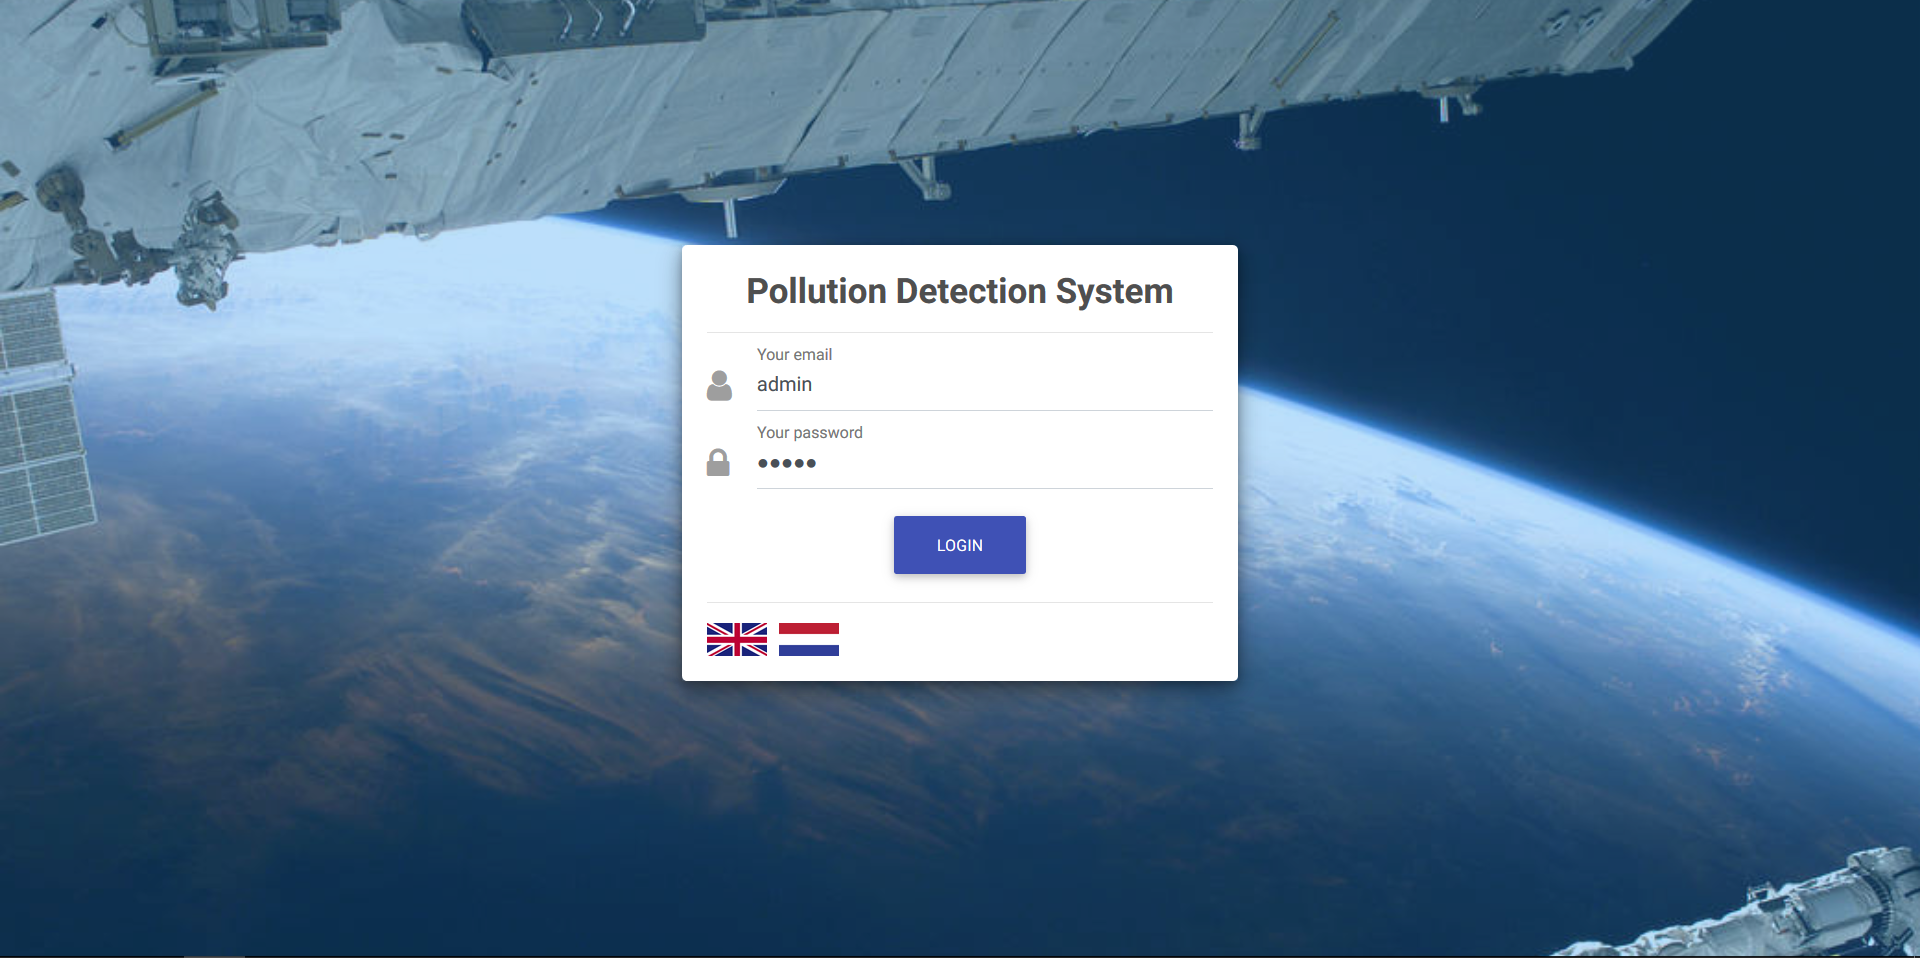
\includegraphics[width=\textwidth]{login}

\noindent
After completing these steps you are being redirected to the homepage.
\newline
On the top of this website there is a navigation bar, which is used to visit the several available pages. These pages include: the home page the map page and the admin page. The latter is only shown if the current user is an admin.
\newline
If you want to log out, simply click the logout button at the very end of the navigation bar.
\newline
Both the login page and home page contain buttons to switch between the languages Dutch and English.

\pagebreak

\subsection{The homepage}
\lipsum[1-2]
% * <thom.de.jong3@hva.nl> 2018-04-23T13:55:33.706Z:
% 
% Information about the homepage will be inserted above after the homepage is finished.
% 
% ^.

\pagebreak

\subsection{The map page}
This page is used for viewing the gathered data. The data is displayed on the map. This map is the website's main feature. It can be used when you want to view the data from the sensorhubs.
\newline
This page features a map which can show you all kinds of data regarding pollution. On the left side there is a sidebar. This sidebar contains many options that can be used, for example: filters with which you can enable the heatmap, light pollution map and more.
\newline
There is also a search bar. With the search bar certain places like cities and towns can be found. Also, it can find a specific location by entering coordinates into the search bar.
~\newline

\subsubsection{The heatmap}
If you want to see the temperature measured by the sensorhubs, this is the right option.
The heatmap shows a representation of the temperature, using colors scaling from bright pink (cold) to red (warm). The colours are displayed on the map as a layer over the standard map.
~\newline\newline
\noindent
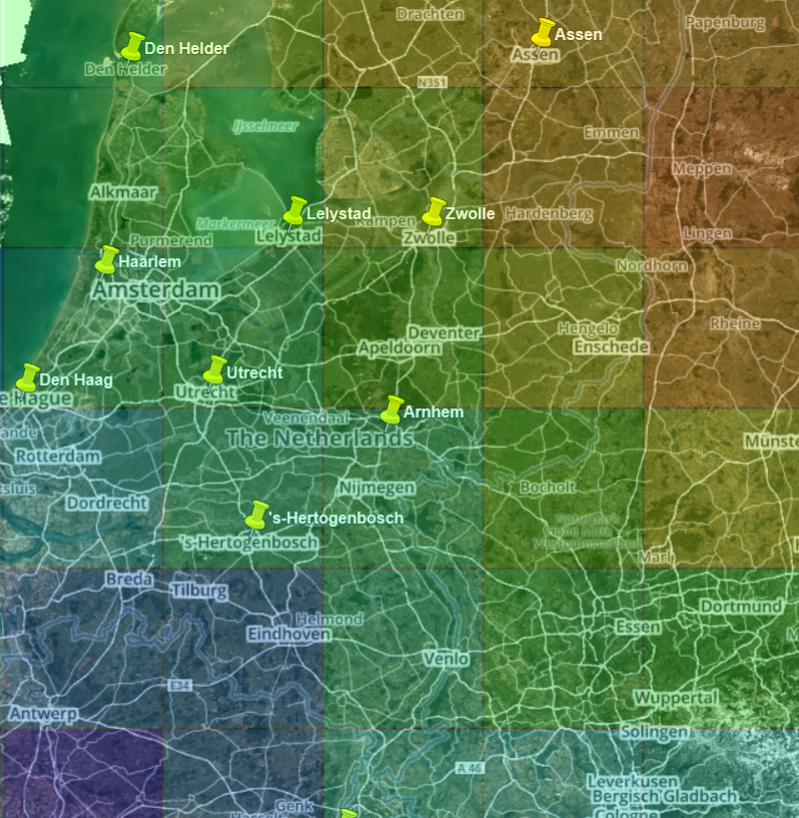
\includegraphics[width=\textwidth]{kaart}
% * <thom.de.jong3@hva.nl> 2018-04-23T13:57:14.016Z:
% 
% Even more maps in the future.
% 
% ^.

\pagebreak

\subsection{The admin page}
This page is used to make changes to the system, e.g. user management. Just like the name says, this page is only available for admins. On this page you can change a user's data or that of a sensorhub.
\newline
This page shows two tables. One table for the Users and one for the sensorhubs. With admin rights the user can change the data inside of these tables.
\newline
For example, the Users table contains data of all the users. With the add button you can add a user and with the delete button behind a specific user you can delete it. Then there is the edit button. The edit button is used to edit the profile of a specific user.
\newline
The sensorhub table simply shows the location of the used sensorhubs with pinpoints.

\pagebreak

\section{Further help}
PLA25 is responsible for making this web application. If any bugs are to be found, please do contact us.
Also contact us if any further help is needed or something is not yet clear.

\end{document}
